\documentclass[letterpaper, 11pt]{article} 

\usepackage{graphicx}
\graphicspath{{images/}}
\usepackage{multicol}
\usepackage{amsmath}
\usepackage{multirow}
\usepackage[spanish,es-tabla]{babel}
\usepackage[utf8]{inputenc}
\usepackage{url}
\usepackage{listings}
\usepackage{siunitx}

\usepackage[font=footnotesize,labelfont=small]{caption}
\captionsetup{width=0.85\linewidth}

\RequirePackage{geometry}
\geometry{margin=2.54cm}

\selectlanguage{spanish}
\setlength{\parindent}{24pt}
\lstset{language=Python}
\lstset{numbers=left, numberstyle=\tiny, stepnumber=1, numbersep=5pt}
\lstset{basicstyle=\scriptsize, keywordstyle=\bfseries}

\title{Simulación numérica de un Ciclotrón}
\author{Nicolas Maldonado Baracaldo}
\author{
Nicolas Maldonado Baracaldo\\
201423809\\
Facultad de Ciencias, Universidad de Los Andes\\
Departamento de Física\\
Aceleradores de Partículas y Sus Aplicaciones\\
Profesor Bernardo Gómez Moreno, Dr. rer. nat.
}
\date{29 de Mayo, 2019}

\begin{document}

\maketitle

\begin{multicols}{2}

\section{Introducción}
El ciclotrón es un tipo de acelerador de partículas que acelera partículas cargadas mediante un campo eléctrico de radiofrecuencia (RF) mientras estas realizan una trayectoria en espiral, desde el centro hacia afuera, bajo la influencia de un campo magnético constante.

El desarrollo del ciclotrón inició en 1929 cuando Ernest O. Lawrence (1901--1958) quiso aplicar los hallazgos de Rolf Widerøe (1902--1996), la aceleración de partículas usando campos RF, de manera sucesiva para alcanzar energías tan altas como las alcanzadas en el momento por otras máquinas de muy alto voltaje. Para evitar tener que usar una larga cadena de electrodos, Lawrence propuso usar un solo electrodo, curvando el haz con un campo magnético para lograr trayectorias circulares de manera que el haz pasara por el electrodo en cada media vuelta.

Entre 1930 y 1932, Lawrence y su equipo en la Universidad de California, Berkeley construyeron los primeros ciclotrones, de 4'' y luego 11'' de diámetro, y lograron aceleraciones de más de 1 MeV, algo nunca antes visto. En 1932, ya trabajando en la construcción de una máquina de 27'', Lawrence patentó su invento, por el cual recibió el premio Nobel en física en 1939.

La era del ciclotrón finalmente llegó a su fin en 1945, cuando se descubrió que estas máquinas estaban limitadas por los efectos relativistas que surgían al alcanzar una cierta energía. En este momento se estaba construyendo un ciclotrón de 184'', el cual se modificó de manera que se actualizara el campo RF a medida que las partículas ganaban energía, manteniendo así la máquina sincronizada. Éste sería el primer sincrociclotrón, máquinas que eventualmente también fueron remplazadas por los sincrotrones, los aceleradores más modernos actualmente.

El principio de funcionamiento del ciclotrón se desprende del movimiento circular de una partícula cargada bajo la influencia de un campo magnético y el hecho de que el periodo de este movimiento es independiente de la velocidad de la partícula (derivación \ref{constantPeriod}). Así, a medida que se aceleran las partículas dentro de la máquina su radio aumenta de manera que el periodo se conserve, dando lugar a un movimiento en espiral.

\begin{equation}
\label{constantPeriod}
    \begin{gathered}
        F_B = q \textbf{v} \times \textbf{B}\\
        F_c = \frac{m v^2}{r}\\
        q v B = \frac{m v^2}{r}\\
        r = \frac{m v}{q B}\\
        T = \frac{2 \pi}{\omega} = \frac{2 \pi r}{v} = \frac{2 \pi m v}{q B v}\\
        T = \frac{2 \pi m}{q B}
    \end{gathered}
\end{equation}

Como se cuenta con un periodo constante, es fácil fijar una frecuencia para el campo RF de manera que en cada paso de las partículas por el electrodo éstas sean aceleradas y no frenadas, la llamada frecuencia de ciclotrón (ecuación \ref{cyclotronFreq}).

\begin{equation}
\label{cyclotronFreq}
    f_C = \frac{q B}{2 \pi m}
\end{equation}

Habiendo fijado esta frecuencia para el campo RF, se asegura que al pasar las partículas por el electrodo, cada medio periodo, éstas estén sometidas a una fuerza de Lorentz por la acción de ambos campos, eléctrico y magnético (ecuación \ref{lorentzF}), la cual continúa curvando la trayectoria (componente magnética) y acelera las partículas (componente eléctrica). Sin embargo, a pesar de que la energía que ganan las partículas viene del campo
eléctrico, se encuentra que la energía de salida del haz está únicamente determinada por la magnitud del campo magnético y por el radio máximo, $R$, del recorrido (derivación \ref{exitEnergy}).

\begin{equation}
\label{lorentzF}
    F_{Lorentz} = q \textbf{E} + q \textbf{v} \times \textbf{B}
\end{equation}

\begin{equation}
\label{exitEnergy}
    \begin{gathered}
        F_B = q \textbf{v} \times \textbf{B}\\
        F_c = \frac{m v^2}{r}\\
        q v B = \frac{m v^2}{R}\\
        v = \frac{q B R}{m}\\
        K = \frac{1}{2} m v^2 = \frac{q^2 B^2 R^2}{2m}
    \end{gathered}
\end{equation}

El diseño básico de un ciclotrón (figura \ref{design}\footnote{Adaptada de El-Saftaway, \textit{Regulating the performance parameters of accelerated particles} por María Alejandra Sánchez.}) consiste en un electroimán con sus polos situados uno arriba y uno abajo de un disco, generando un campo magnético uniforme al interior de éste. El disco en sí está dividido en dos mitades semicirculares llamadas Ds (o frecuentemente ''dees'' en inglés) separadas por una pequeña brecha entre sus segmentos lineares, espacio en el cual se encuentra un campo eléctrico de radiofrecuencia y espacialmente uniforme creado al conectar cada D a una terminal de un oscilador con la frecuencia adecuada (ecuación \ref{cyclotronFreq}).\\

\begin{center}
    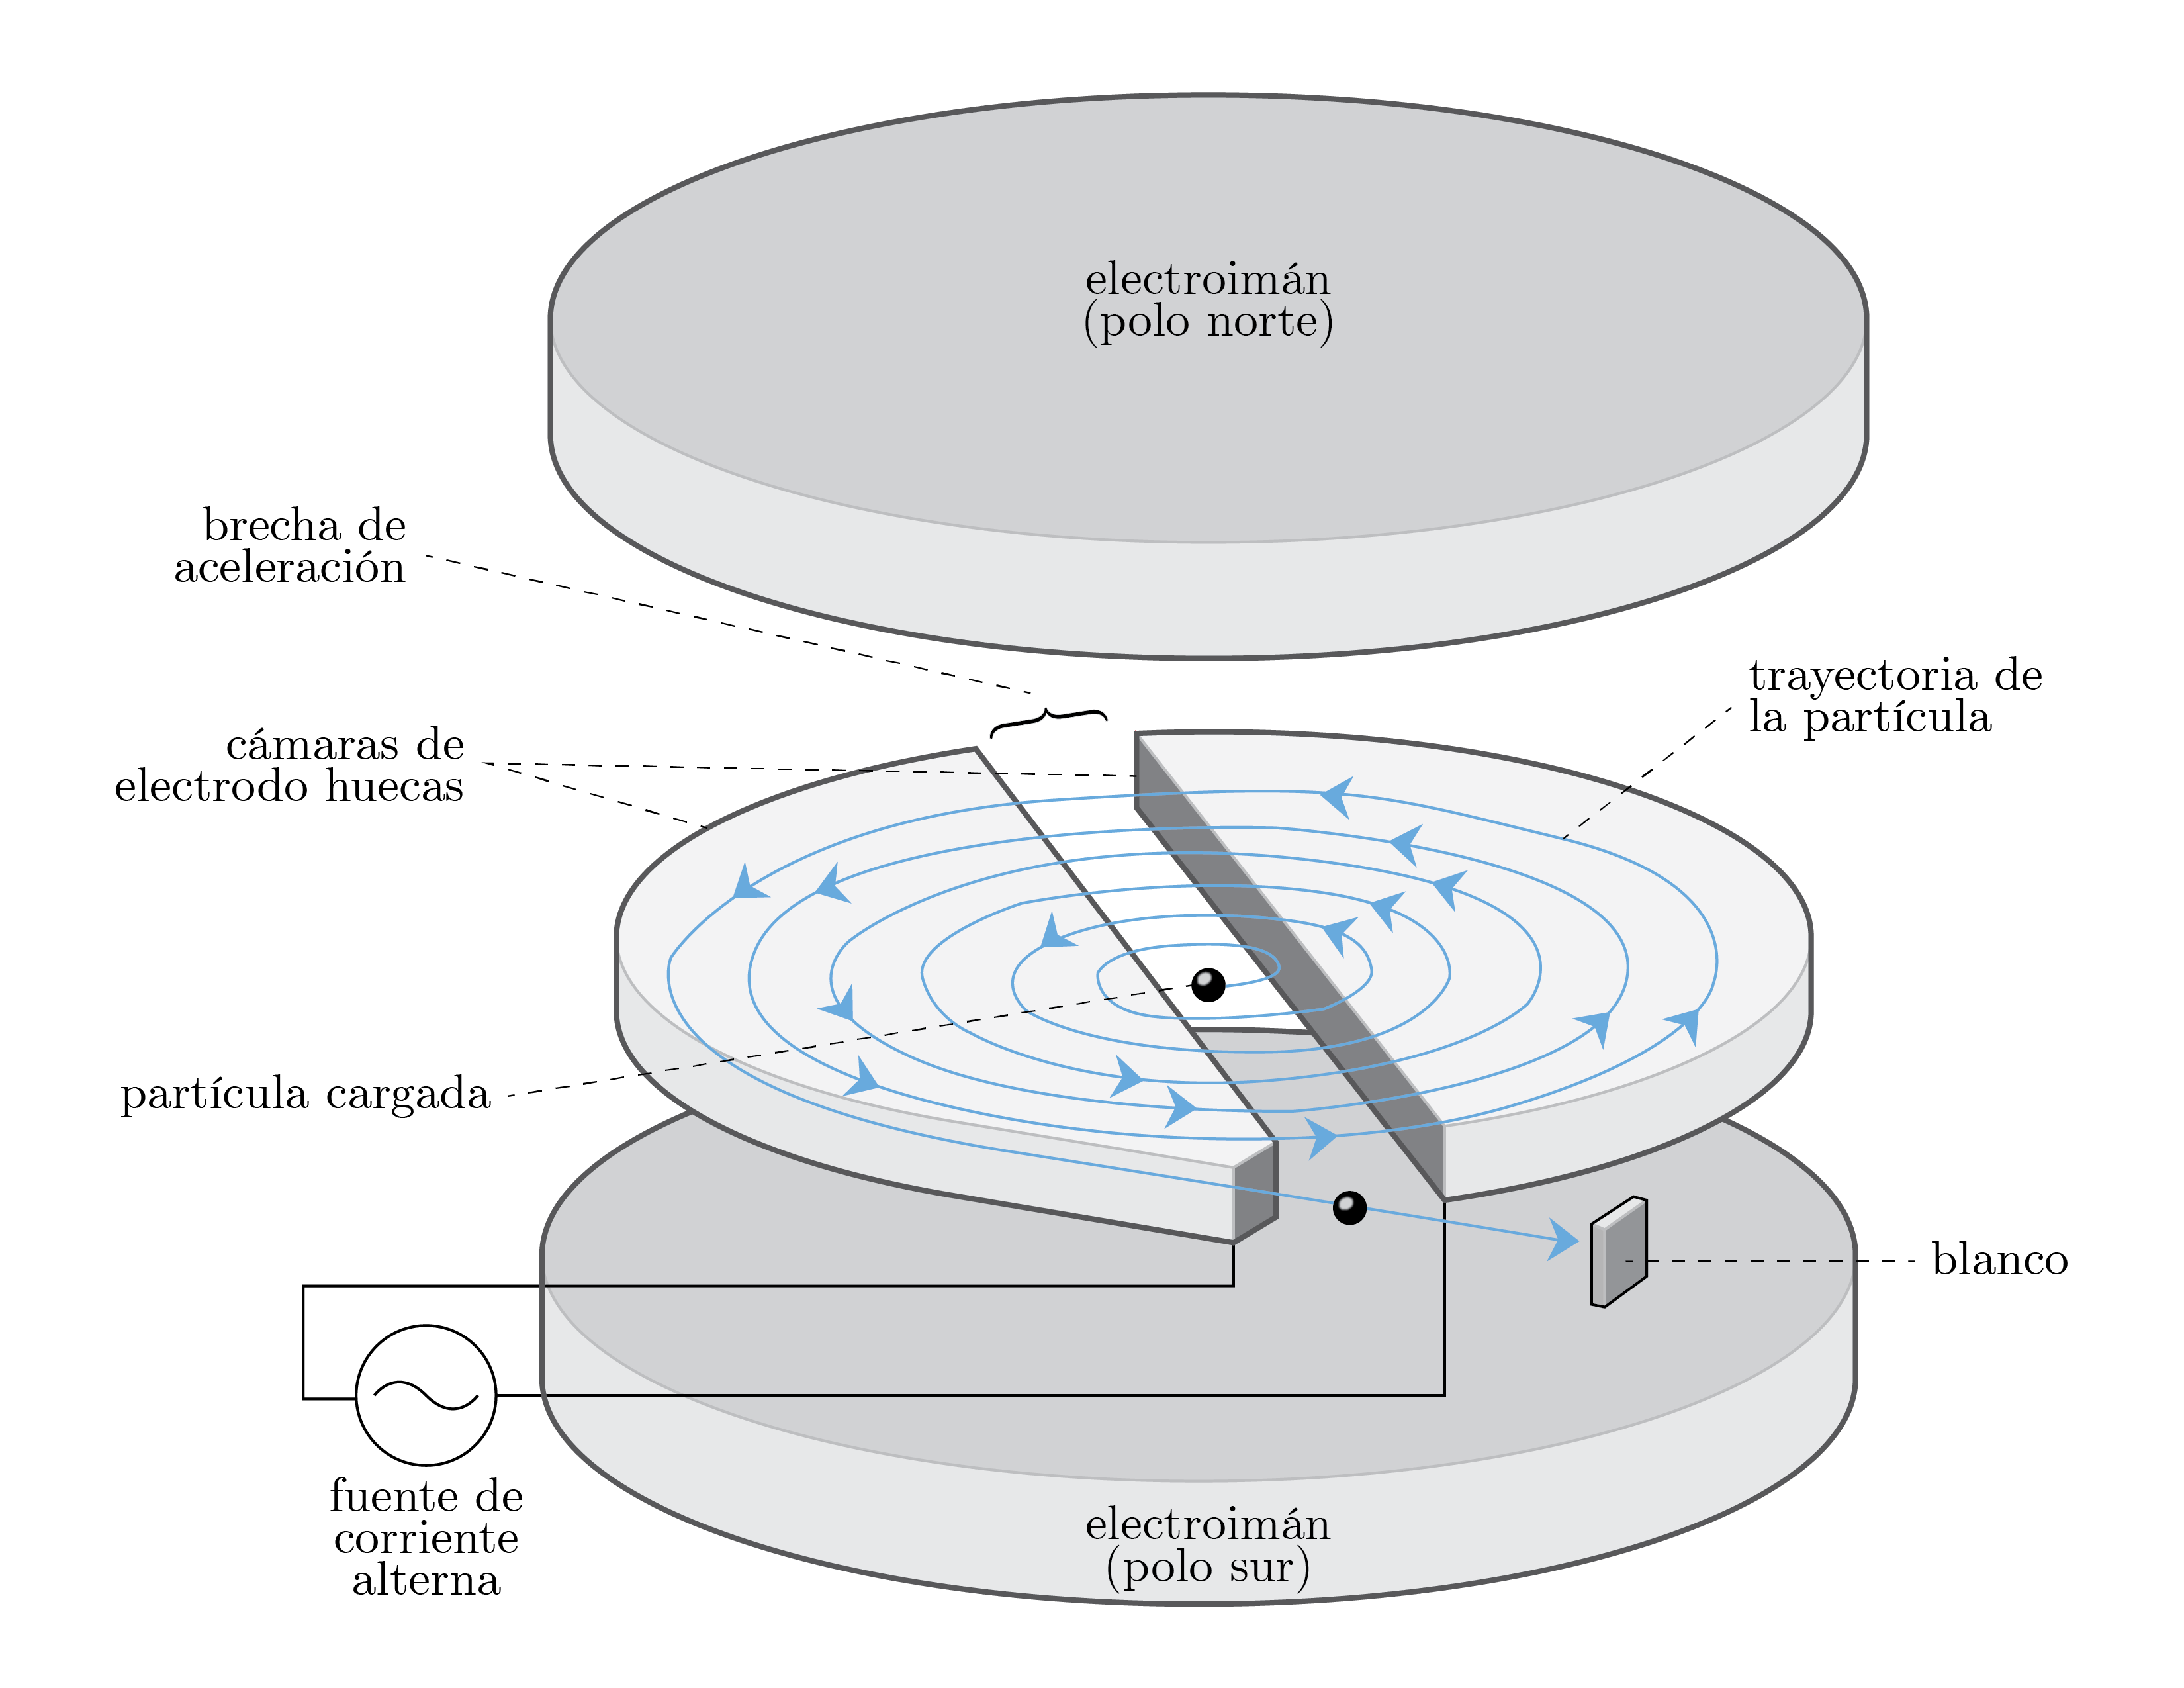
\includegraphics[width=0.5\textwidth]{design.png}
    \captionof{figure}{Diseño básico de un ciclotrón}
    \label{design}
\end{center}

\section{Método}
Se escribió un código que permitiera simular numéricamente el funcionamiento de un ciclotrón, tomando como valores de entrada los parametros de la máquina misma, los parametros de la partícula (protón), y algunos parametros para la simulación ---la posición y velocidad iniciales de la partícula, el tiempo de operación a simular, y el número total de puntos a tomar.\\

Se definen dos funciones para usar durante la ejecución de la simulación. La primera, \textit{F\_Lorentz()}, calcula la fuerza de Lorentz correspondiente a la posición, la velocidad, y el tiempo ingresados como parametros, si bien la velocidad es un parametro necesario en el cálculo de esta fuerza (ecuación \ref{lorentzF}), y el tiempo es el parametro que determina la amplitud del campo eléctrico según la frecuencia de ciclotrón (ecuación \ref{cyclotronFreq}), la posición se ingresa como el parametro en dos funciones de Heaviside que sirven para incluir o excluir, según sea el caso, la componente eléctrica de la fuerza, puesto que ésta solo la experimentarán las partículas cuando pasan entre las Ds.

La segunda función, \textit{RK4()}, utiliza el más utilizado método iterativo de Runge-Kutta, el de cuarto orden, para aproximar las soluciones de una ecuación diferencial ordinaria de segundo orden con discretización temporal. Puesto que el método puede usarse para aproximar soluciones a sistemas de la forma (\ref{difEq}), se reconoce que se puede aplicar a la simulación numérica de un ciclotrón, teniendo en cuenta que \(\textbf{r}(t)\), las posiciones, pueden hallarse a partir de \(\textbf{v}(t, \textbf{r}) = \mathbf{\dot{r}}(t, \textbf{r})\), las velocidades, y estas a su vez pueden hallarse a partir de \(\textbf{a}(t, \textbf{r}, \textbf{v}) = \mathbf{\dot{v}}(t, \textbf{r}, \textbf{v})= \mathbf{F_{Lorentz}}(t, \textbf{r}, \textbf{v})/m\), las aceleraciones calculadas directamente de las fuerzas de Lorentz que apliquen en cada punto de la trayectoria, todo con pasos de tamaño $dt$.

\begin{equation}
\label{difEq}
    \begin{gathered}
        \dot{y_1} = y_2\\
        \dot{y_2} = f(t, y_1, y_2)
    \end{gathered}
\end{equation}

Así pues, el código toma los parámetros de entrada para inicializar la posición, la velocidad, y la aceleración, crea un arreglo para la discretización temporal con $N$ elementos temporales en el rango [0, $t\_max$] con separación $dt$, y procede a iterar sobre ellos. En cada iteración se actualizan $r$, $v$, y $a$, a partir de los cuales se van guardando en sus respectivos arreglos las posiciones en $x$ y en $y$, los momentos en $x$ y en $y$, y los radios de la trayectoria calculados a partir de la posición, $r_{xy}$ (método geométrico) y del momento, $r_p$ (método válido para ciclotrones según ecuación \ref{momentumR}).

\begin{equation}
\label{momentumR}
    r(t) = \frac{\lVert \textbf{p} (t) \rVert}{q B}
\end{equation}

Finalmente se usan los arreglos creados para generar una gráfica de $y$ vs. $x$, mostrando la trayectoria de las partículas, así como gráficas de $x$ vs. $p_x$, $y$ vs. $p_y$, y $r_{xy}$ vs. $r_p$.

\end{multicols}

\section{Código}
A continuación se muestra en su totalidad el código empleado, escrito en Python 3.6:\\

\begin{lstlisting}
#################### Numerical Simulation of a Cyclotron ####################
### Nicolas Maldonado Baracaldo
### 201423809
#############################################################################

import numpy as np
import matplotlib.pyplot as plt

### Cyclotron parameters: ###
E = np.array([6000000,0,0]) #Electric field
B = np.array([0,0,-1.64])   #Magnetic field
R = 0.923                   #Radius
d = 0.120                   #Distance between dees

### Particle parameters: ###
q = 1.6021766*10**-19 #Particle charge
m = 1.6726219*10**-27 #Particle mass

### Simulation parameters: ###
r_0 = np.array([0,0.05,0]) #Initial position
v_0 = np.array([100,0,0])  #Initial velocity
t_max = 1.3*10**-6         #Simulation running time
N = 10000                  #Number of samples for simulation

### Function to calculate Lorentz force: ###
def F_Lorentz(r, v, t):
    return q*E*np.cos((q*B[2]/m)*t)*np.heaviside(r[0]+d/2, 1)*np.heaviside(-r[0]+d/2, 1)\
            + q*np.cross(v, B)
#end of F_Lorentz() function

### Function to update r, v, a via 4th order Runge-Kutta: ###
def RK4(t):
    global r
    global v
    global a
    global dt
    
    #First step:
    k1 = v
    l1 = a
    
    #Second step:
    k2 = v + dt/2*l1
    l2 = F_Lorentz(r+dt/2*k1, k2, t+dt/2)/m
    
    #Third step:
    k3 = v + dt/2*l2
    l3 = F_Lorentz(r+dt/2*k2, k3, t+dt/2)/m
    
    #Fourth step:
    k4 = v + dt*l3
    l4 = F_Lorentz(r+dt*k3, k4, t+dt)/m
    
    #Averages:
    k = (k1 + 2*k2 + 2*k3 + k4)/6
    l = (l1 + 2*l2 + 2*l3 + l4)/6

    #Update acceleration:
    a = F_Lorentz(r, v, t+dt)/m
    #Update velocity
    v = v + dt*l
    #Update position
    r = r + dt*k
#end of RK4() function

t = np.linspace(0,t_max,N) #Times array
dt = t[1] - t[0]           #Time step
r = r_0                    #Set initial position
v = v_0                    #Set initial velocity
a = F_Lorentz(r, v, 0)/m   #Set initial acceleration

x = np.array([r[0]]) #X positions array
y = np.array([r[1]]) #Y positions array

p_x = np.array([m*v[0]/(5.36*10**-22)]) #X momenta array
p_y = np.array([m*v[1]/(5.36*10**-22)]) #Y momenta array

r_xy = np.array([np.sqrt(r[0]**2 + r[1]**2)])                  #Position-based radii array
r_p = np.array([np.sqrt((m*v[0])**2 + (m*v[1])**2)/(-q*B[2])]) #Momentum-based radii array

### Loop over times ###
for i in range(1,t.size):
    #Update variables:
    RK4(t[i-1])
    
    #Store positions:
    x = np.append(x, [r[0]])
    y = np.append(y, [r[1]])
    
    #Store momenta:
    p_x = np.append(p_x, [m*v[0]/(5.36*10**-22)])
    p_y = np.append(p_y, [m*v[1]/(5.36*10**-22)])
    
    #Store radii:
    r_xy = np.append(r_xy, [np.sqrt(r[0]**2 + r[1]**2)])
    r_p = np.append(r_p, [np.sqrt((m*v[0])**2 + (m*v[1])**2)/(-q*B[2])])
    
    #Stop loop when approaching radius:
    if r[0] > 0.935*R:
        break
    #end if statement
#end of for loop

#Fix null acceleration:
a = np.array([0,0,0])

### Loop over remaining times ###   
for i in range(x.size,t.size):
    #Update position:
    r = r + dt*v
    
    #Store positions:
    x = np.append(x, [r[0]])
    y = np.append(y, [r[1]])
    
    #Store momenta:
    p_x = np.append(p_x, [m*v[0]/(5.36*10**-22)])
    p_y = np.append(p_y, [m*v[1]/(5.36*10**-22)])
    
    #Store radii:
    r_xy = np.append(r_xy, [np.sqrt(r[0]**2 + r[1]**2)])
    r_p = np.append(r_p, [np.sqrt((m*v[0])**2 + (m*v[1])**2)/(-q*B[2])])
    
    #Stop loop once radius is reached:
    if r[1] > R:
        break
    #end if statement
#end of for loop
   
p_l = np.linspace(0.5211189*np.pi,1.4788811*np.pi,100)   #Angles for left dee
x_l = np.append([-d/2,-d/2],0.906996*np.cos(p_l))        #X coordinates of left dee
y_l = np.append([-0.86,0.95],0.906996*np.sin(p_l)+0.045) #Y coordinates of left dee

p_r = np.linspace(-0.4788811*np.pi,0.4788811*np.pi,100)  #Angles for right dee
x_r = np.append([d/2,d/2],0.906996*np.cos(p_r))          #X coordinates of right dee
y_r = np.append([0.95,-0.86],0.906996*np.sin(p_r)+0.045) #Y coordinates of right dee

#Plot y positions vs. x positions:
plt.figure(figsize=[12,12])
plt.rc('xtick',labelsize=12)
plt.rc('ytick',labelsize=12)
plt.xlabel(r'$x$ (m)',fontsize=14)
plt.ylabel(r'$y$ (m)',fontsize=14)
plt.plot(x,y,color='#74AAE1',linewidth=2)
plt.plot(x_l,y_l,color='grey')
plt.plot(x_r,y_r,color='grey')
plt.savefig('path.png')
plt.close()

#Plot x positions vs. x momenta:
plt.figure(figsize=[12,12])
plt.rc('xtick',labelsize=12)
plt.rc('ytick',labelsize=12)
plt.xlabel(r'$p_x$ (MeV/c)',fontsize=14)
plt.ylabel(r'$x$ (m)',fontsize=14)
plt.plot(p_x,x,color='#74AAE1',linewidth=2)
plt.savefig('momentum_x.png')
plt.close()

#Plot y positions vs. y momenta:
plt.figure(figsize=[12,12])
plt.rc('xtick',labelsize=12)
plt.rc('ytick',labelsize=12)
plt.xlabel(r'$p_y$ (MeV/c)',fontsize=14)
plt.ylabel(r'$y$ (m)',fontsize=14)
plt.plot(p_y,y,color='#74AAE1',linewidth=2)
plt.savefig('momentum_y.png')
plt.close()

#Plot position-based radii vs. momentum-based radii:
plt.figure(figsize=[12,12])
plt.rc('xtick',labelsize=12)
plt.rc('ytick',labelsize=12)
plt.xlabel(r'$r_p$ (m)',fontsize=14)
plt.ylabel(r'$r_{xy}$ (m)',fontsize=14)
plt.plot(r_p,r_xy,color='#74AAE1',linewidth=2)
plt.savefig('radii.png')
plt.close()
\end{lstlisting}

\begin{multicols}{2}

\section{Parámetros}
Se ingresaron en el código todos los parámetros necesarios para la simulación numérica, como se explica en la sección 2, separados en tres partes: parámetros del ciclotrón (\ref{cyclotronP}), parámetros de la partícula (\ref{particleP}), y parámetros iniciales para la simulación (\ref{simP}).

\begin{equation}
\label{cyclotronP}
    \begin{cases}
        E = 6 \hspace{3pt} \text{\small{MV}} \hspace{18pt} \text{\footnotesize{Magnitud campo eléctrico}}\\
        B = 1.64 \hspace{3pt} \text{\small{T}} \hspace{14pt} \text{\footnotesize{Magnitud campo magnético}}\\
        R = 0.923 \hspace{3pt} \text{\small{m}} \hspace{8pt} \text{\footnotesize{Radio máximo}}\\
        d = 120 \hspace{3pt} \text{\small{mm}} \hspace{10pt} \text{\footnotesize{Separación entre las Ds}}
    \end{cases}
\end{equation}

\begin{equation}
\label{particleP}
    \begin{cases}
        q = \num{1.602e-19} \hspace{3pt} \text{\small{C}} \hspace{15pt} \text{\footnotesize{Carga del protón}}\\
        m = \num{1.673e-27} \hspace{3pt} \text{\small{kg}} \hspace{8pt} \text{\footnotesize{Masa del protón}}\\
    \end{cases}
\end{equation}

\begin{equation}
\label{simP}
    \begin{cases}
        r_0 = 0.05 \hspace{3pt} \text{\small{m}} \hspace{46pt} \text{\footnotesize{Posición en $y$}}\\
        v_0 = 100 \hspace{3pt} \text{\small{m/s}} \hspace{39pt} \text{\footnotesize{Velocidad en $x$}}\\
        t_{max} = \num{1.3e-6} \hspace{3pt} \text{\small{s}} \hspace{8pt} \text{\footnotesize{Tiempo máximo}}\\
        N = 10000 \hspace{49pt} \text{\footnotesize{Número de puntos}}
    \end{cases}
\end{equation}

\section{Resultados}
Como se detalla en la sección 2, la última parte del código genera cuatro gráficas a partir de los valores que arroja la aproximación numérica realizada. La primera de ellas, la de la trayectoria de las partículas (figura \ref{path}), sirve principalmente para confirmar la precisión de la simulación pues la trayectoria de las partículas en un ciclotrón es bien conocida. En efecto se logra la trayectoria en espiral con radio creciente que se espera y puede además comprobarse que los detalles de esta trayectoria varían al variar los parámetros de entrada de acuerdo al funcionamiento elucidado en la sección 1.

\begin{center}
    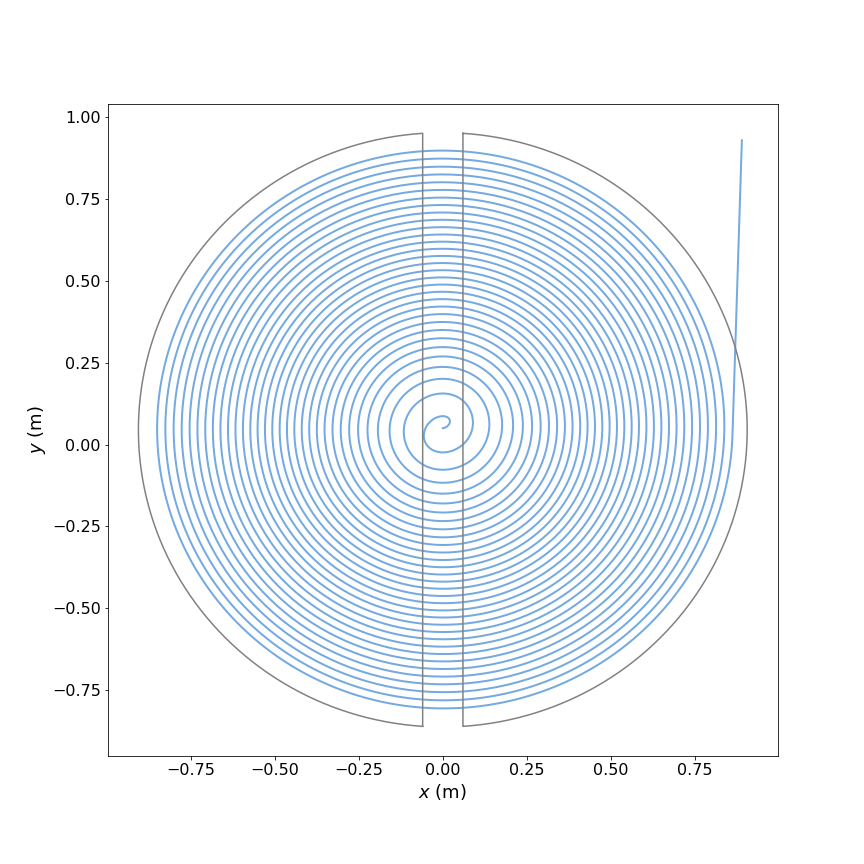
\includegraphics[width=0.5\textwidth]{path.png}
    \captionof{figure}{Trayectoria de las partículas.}
    \label{path}
\end{center}

Habiendo comprobado ya la validez del modelo pueden ahora analizarse las demás gráficas con el fin de entender más sobre este acelerador de partículas. Las gráficas de posición vs. momento (figuras \ref{momentumX} y \ref{momentumY}) permiten ver precisamente cómo van ganando energía las partículas a lo largo de su recorrido y cómo se relaciona esto con la trayectoria que trazan. A medida que aumenta la energía de las partículas, es decir, que ganan momento lineal, visto en este caso en su componente en $x$ y en su componente en $y$, y estando sometidas las partículas al mismo campo magnético, las distancias que logran alcanzar sobre cada eje aumentan igualmente. De igual manera, dada la trayectoria misma que siguen las partículas, éstas oscilan sobre cada eje entre los valores positivo y negativo de esta distancia máxima, y de igual manera el vector momento rota, haciendo oscilar cada uno de sus componentes entre los valores positivo y negativo del momento neto. Este comportamiento resulta, finalmente, en que el par momento-posición, sobre un mismo eje dado, evolucione en el tiempo trazando una espiral como la de la trayectoria de las partículas.

\begin{center}
    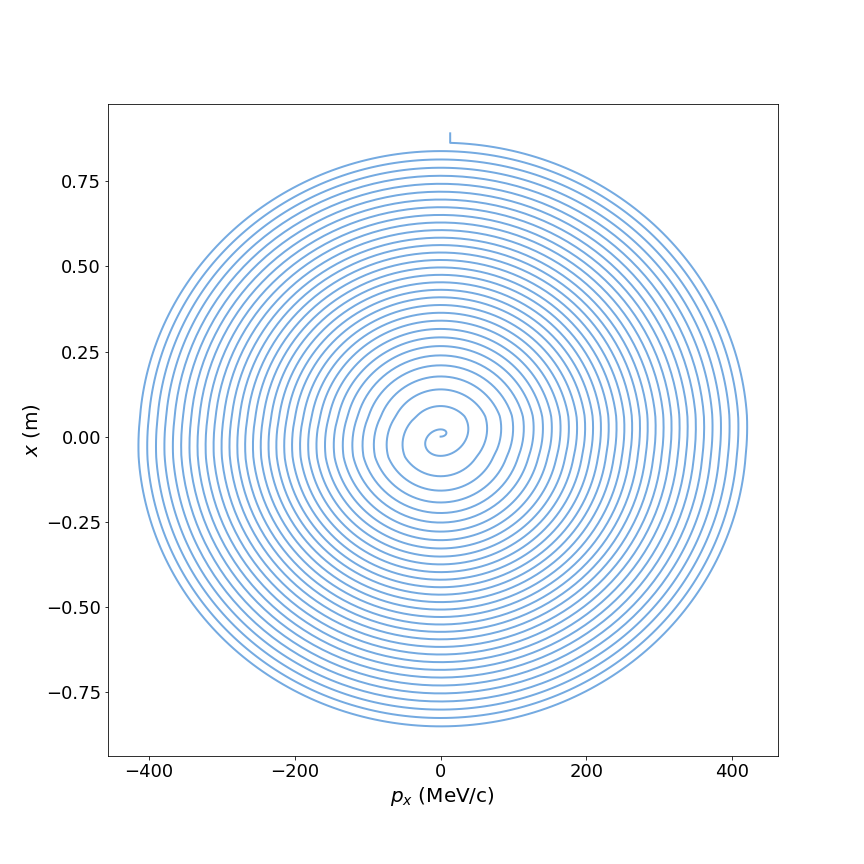
\includegraphics[width=0.5\textwidth]{momentum_x.png}
    \captionof{figure}{Posición en $x$ vs. momento en $x$.}
    \label{momentumX}
\end{center}

\begin{center}
    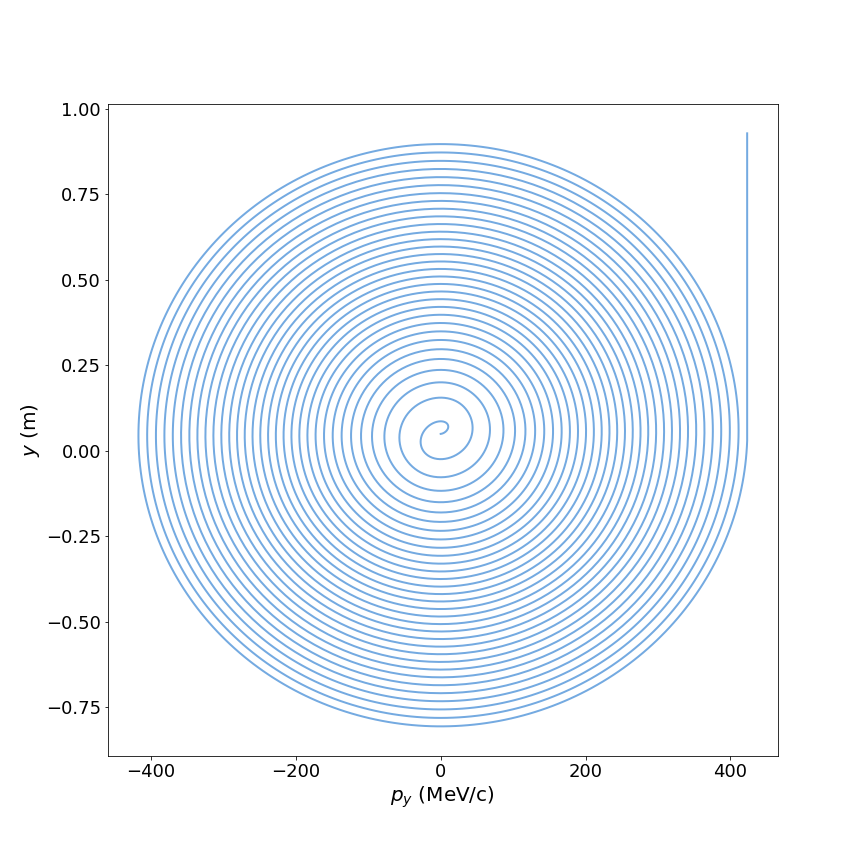
\includegraphics[width=0.5\textwidth]{momentum_y.png}
    \captionof{figure}{Posición en $y$ vs. momento en $y$.}
    \label{momentumY}
\end{center}

Finalmente, la última gráfica (figura \ref{radii}) permite comparar el radio real del recorrido de las partículas en cada instante de tiempo, es decir, el calculado a partir de su posición, con el radio esperado según la energía alcanzada por la partícula hasta dicho instante. El patrón que se observa responde simplemente a la manera pulsada en que el ciclotrón acelera las partículas, pues el campo eléctrico les transfiere suficiente energía para completar un recorrido de mayor radio antes de que efectivamente lo hagan, pero esta transferencia de energía solo se da en unos momentos del recorrido, permitiendo que el radio real aumente durante el resto del mismo hasta llegar a coincidir ambos. Este comportamiento se repite periódicamente, en cada medio círculo que completan las partículas.

\begin{center}
    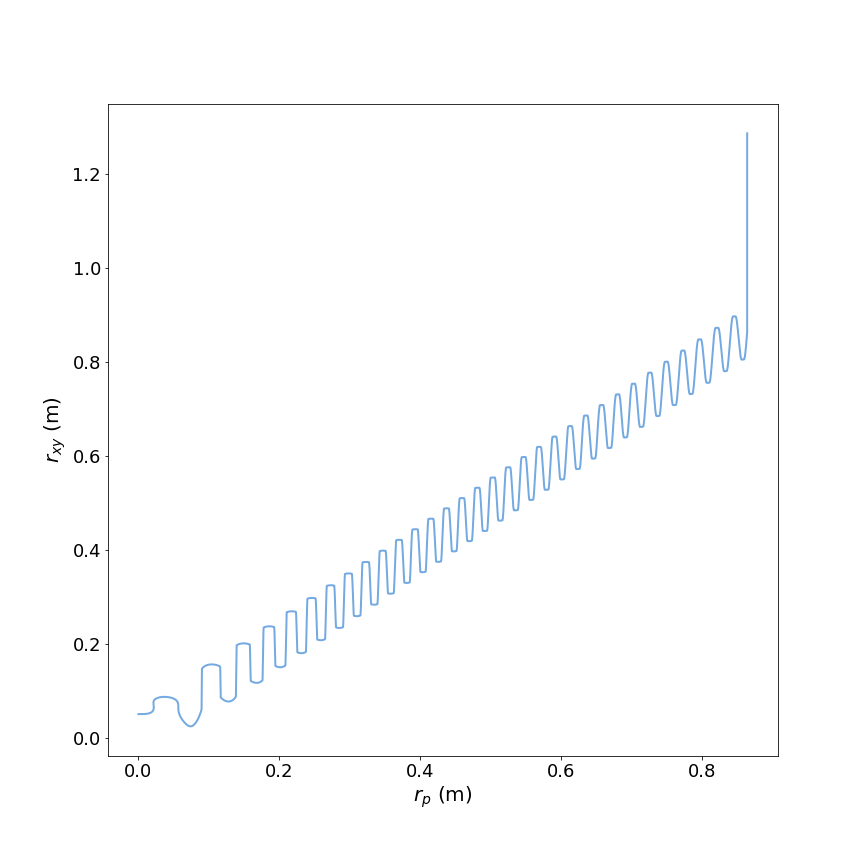
\includegraphics[width=0.5\textwidth]{radii.png}
    \captionof{figure}{Comparación de radios.}
    \label{radii}
\end{center}

\section{Conclusiones}
El ciclotrón fue un acelerador de partículas de gran importancia histórica, permitiendo alcanzar energías nunca antes vistas y llevando eventualmente al desarrollo del sincrotrón, el que hoy en día es el más moderno acelerador, y aún hoy en día se usan ampliamente los ciclotrones. Es por esto que una parte esencial de aprender sobre aceleradores de partículas es aprender sobre el ciclotrón y entender a fondo el principio detrás de su funcionamiento. Si bien este funcionamiento puede ser explicado con relativa facilidad, y puede ésto apoyarse por todas las ecuaciones pertinentes, probablemente no hay mejor forma de entender verdaderamente un ciclotrón que simularlo por medio de métodos numéricos, pudiendo así ver paso a paso cómo opera la máquina y cómo pueden manipularse los diversos parámetros de la misma para lograr los resultados que se deseen.

\begin{thebibliography}{9}
    \bibitem{history}
    ''A Brief Historical Review of the Invention of the Cyclotron.'' Koeth Cyclotron. Marzo 10, 2016. Consultado Mayo 28, 2019. http://koethcyclotron.org/?page\_id=54.
    
    \bibitem{diagram}
    El-Shaftaway, Ashraf. ''Regulating the Performance Parameters of Accelerated Particles.'' Ph.D. thesis, 2013.
    
    \bibitem{Runge-Kutta}
    ''Runge-Kutta for a System of Differential Equations.'' Runge-Kutta for a System. Consultado Mayo 28, 2019. https://www.nsc.liu.se/~boein/f77to90/rk.html.
    
    \bibitem{latexcompanion}
    ''Theory of Operation.'' Koeth Cyclotron. Marzo 10, 2016. Consultado Mayo 28, 2019. http://koethcyclotron.org/?page\_id=64.
\end{thebibliography}

\end{multicols}
\end{document}